\chapter{Lecture 27}
\lhead{March 25, 2015}
\chead{21-366 Lambda Calculus Lecture 27}
\rhead{Brian Jacobs}
\pagestyle{fancy}

\section{B\"ohm Trees}
\textbf{Definition:} A B\"ohm tree is a finitely branching tree whose nodes are labeled
\begin{enumerate}[(1)]
  \item With a \l{} prefix and a head variable
    \begin{equation*}
      \l x_1\ldots x_n.x_i\ \ i\in \mathbb{N}
    \end{equation*}
  \item If the tree is a leaf, then
    \begin{equation*}
      \bot
    \end{equation*}
\end{enumerate}
We associate to each term $X$ a B\"ohm tree. If $X$ is unsolvable (that is, it has no head-normal form - by Wadsworth's Theorem), then the B\"ohm tree of $X$ is simply $\bot$. However if $X$ has a head normal form $\l x_1\ldots x_n . x_iX_1\ldots X_m$, then the B\"ohm tree of $X$ should be:
\begin{center}
  \begin{tikzpicture}
    \Tree[.$\l x_1\ldots x_n.x_i$ [.$BT(X_1)$ ] [.$\ldots$ ] [.$BT(X_m)$ ] ]
  \end{tikzpicture}
\end{center}

\textbf{Claim:} If $T = \hbox{BT}(X)$, then $T$ has finitely many free variables.\\

\textbf{Barendreight's theorem:} If a finitely bounded B\"ohm tree has finitely many free variables then it is the B\"ohm tree of a term. TODO: FIGURE OUT WHAT THIS IS CALLED AND FILL IT OUT.

\subsection{A Useful Ordering of B\"ohm Trees}
We say that $T_1 \sqsubseteq T_2$ if you can take $T_1$ and replace (possibly infintely many) $\bot$ nodes with arbitrary other B\"ohm trees.\\

Remark: $\sqsubseteq$ is a partial ordering. It is reflexive: $T_1 \sqsubseteq T_1$. It is transitive.\\

Remark: $T$ is finite.\\

Definition: $T_1$ and $T_2$ are \textbf{compatible} if there exists $T_1 \sqsubseteq T_3 \sqsupseteq T_2$.\\

Suppose that we have closed terms $M,N$ and a closed term $F$ such that $FM =_\beta K$ and $FN =_\beta K_*$. Then there exists a term with finite B\"ohm tree $M_1$ and a term $N_1$ with finite B\"ohm tree such that $BT(M_1) \sqsubseteq BT(M)$. We say that $M_1$ is an \textbf{approximation} of $M$. The same is true of $N$: $BT(N_1) \sqsubseteq BT(N)$.\\

Stated another way: IF there exists a term $F$ that can differentiate between $M$ and $N$, then it only needs to use a finite amount of the B\"ohm trees of $M$ and $N$ to do so. This idea is called \textbf{continuity}. This in particular is a weak form of continuity. Theoretically, we can put anything in place of $K$ and $K_*$, but if they have different B\"ohm trees, the theorem gets really hard to prove.\\


We have $FM =_\beta K$ and $FN =_\beta K_*$, so
\begin{eqnarray*}
  FMxy \stackrel{\hbox{head reduction}}{\twoheadrightarrow} x\\
  FNxy \stackrel{\hbox{head reduction}}{\twoheadrightarrow} y\\
\end{eqnarray*}

\textbf{Definition:} The levels of a B\"ohm tree. The root of a B\"ohm tree is level 1. Every subB\"ohm tree is of level 2.\\

\textbf{Proof:} Suppose that $FM =_\beta K$. THen $FMxy =_\beta x$. So $FMxy \twoheadrightarrow_\beta x$. Then there is an assignment of potentials $(FMxy)^{\alpha} \twoheadrightarrow_\beta x^{\alpha'}$. This is a normal form. By our theorem of Strong Normalization and uniqueness of normal form, we know that any reduction sequence of terms with potential beginning with $(FMxy)^\alpha$ must terminate in the term $x^{\alpha'}$. We can pick the reduction sequence which first puts $M$ in normal form as a term with potential. We call this new term $M'$.
\begin{equation*}
  M' = \l x_1\ldots x_n . \left\{
  \begin{tabular}{l}
    $x_i X_1\ldots X_m$\\
    or\\
    $(\l x X)^{0}X_1\ldots X_m$
  \end{tabular}
  \right.
\end{equation*}
If we have our first case case, the redex must be projected. In our second case we have a term with potential $0$ so, we simply replace it with $\bot$, as not it nor its residual can be constracted.\\

So $M_1$ is the result of replacing terms of the second kind with bottom. The B\"ohm tree of $M_1$ is therefore clearly less than or equal to the B\"ohm tree of $M$. $BT(M_1) \sqsubseteq BT(M)$.\\

It is then sufficient to consider terms with finite B\"ohm trees. \qqed\\

Next time we will codify properties of unsolvable terms.